\documentclass[]{article}
\usepackage{lmodern}
\usepackage{amssymb,amsmath}
\usepackage{ifxetex,ifluatex}
\usepackage{fixltx2e} % provides \textsubscript
\ifnum 0\ifxetex 1\fi\ifluatex 1\fi=0 % if pdftex
  \usepackage[T1]{fontenc}
  \usepackage[utf8]{inputenc}
\else % if luatex or xelatex
  \ifxetex
    \usepackage{mathspec}
  \else
    \usepackage{fontspec}
  \fi
  \defaultfontfeatures{Ligatures=TeX,Scale=MatchLowercase}
\fi
% use upquote if available, for straight quotes in verbatim environments
\IfFileExists{upquote.sty}{\usepackage{upquote}}{}
% use microtype if available
\IfFileExists{microtype.sty}{%
\usepackage{microtype}
\UseMicrotypeSet[protrusion]{basicmath} % disable protrusion for tt fonts
}{}
\usepackage[margin=1in]{geometry}
\usepackage{hyperref}
\hypersetup{unicode=true,
            pdftitle={Effect of Vitamin C on Tooth Growth in Guinea Pigs},
            pdfauthor={Aslak},
            pdfborder={0 0 0},
            breaklinks=true}
\urlstyle{same}  % don't use monospace font for urls
\usepackage{color}
\usepackage{fancyvrb}
\newcommand{\VerbBar}{|}
\newcommand{\VERB}{\Verb[commandchars=\\\{\}]}
\DefineVerbatimEnvironment{Highlighting}{Verbatim}{commandchars=\\\{\}}
% Add ',fontsize=\small' for more characters per line
\usepackage{framed}
\definecolor{shadecolor}{RGB}{248,248,248}
\newenvironment{Shaded}{\begin{snugshade}}{\end{snugshade}}
\newcommand{\KeywordTok}[1]{\textcolor[rgb]{0.13,0.29,0.53}{\textbf{#1}}}
\newcommand{\DataTypeTok}[1]{\textcolor[rgb]{0.13,0.29,0.53}{#1}}
\newcommand{\DecValTok}[1]{\textcolor[rgb]{0.00,0.00,0.81}{#1}}
\newcommand{\BaseNTok}[1]{\textcolor[rgb]{0.00,0.00,0.81}{#1}}
\newcommand{\FloatTok}[1]{\textcolor[rgb]{0.00,0.00,0.81}{#1}}
\newcommand{\ConstantTok}[1]{\textcolor[rgb]{0.00,0.00,0.00}{#1}}
\newcommand{\CharTok}[1]{\textcolor[rgb]{0.31,0.60,0.02}{#1}}
\newcommand{\SpecialCharTok}[1]{\textcolor[rgb]{0.00,0.00,0.00}{#1}}
\newcommand{\StringTok}[1]{\textcolor[rgb]{0.31,0.60,0.02}{#1}}
\newcommand{\VerbatimStringTok}[1]{\textcolor[rgb]{0.31,0.60,0.02}{#1}}
\newcommand{\SpecialStringTok}[1]{\textcolor[rgb]{0.31,0.60,0.02}{#1}}
\newcommand{\ImportTok}[1]{#1}
\newcommand{\CommentTok}[1]{\textcolor[rgb]{0.56,0.35,0.01}{\textit{#1}}}
\newcommand{\DocumentationTok}[1]{\textcolor[rgb]{0.56,0.35,0.01}{\textbf{\textit{#1}}}}
\newcommand{\AnnotationTok}[1]{\textcolor[rgb]{0.56,0.35,0.01}{\textbf{\textit{#1}}}}
\newcommand{\CommentVarTok}[1]{\textcolor[rgb]{0.56,0.35,0.01}{\textbf{\textit{#1}}}}
\newcommand{\OtherTok}[1]{\textcolor[rgb]{0.56,0.35,0.01}{#1}}
\newcommand{\FunctionTok}[1]{\textcolor[rgb]{0.00,0.00,0.00}{#1}}
\newcommand{\VariableTok}[1]{\textcolor[rgb]{0.00,0.00,0.00}{#1}}
\newcommand{\ControlFlowTok}[1]{\textcolor[rgb]{0.13,0.29,0.53}{\textbf{#1}}}
\newcommand{\OperatorTok}[1]{\textcolor[rgb]{0.81,0.36,0.00}{\textbf{#1}}}
\newcommand{\BuiltInTok}[1]{#1}
\newcommand{\ExtensionTok}[1]{#1}
\newcommand{\PreprocessorTok}[1]{\textcolor[rgb]{0.56,0.35,0.01}{\textit{#1}}}
\newcommand{\AttributeTok}[1]{\textcolor[rgb]{0.77,0.63,0.00}{#1}}
\newcommand{\RegionMarkerTok}[1]{#1}
\newcommand{\InformationTok}[1]{\textcolor[rgb]{0.56,0.35,0.01}{\textbf{\textit{#1}}}}
\newcommand{\WarningTok}[1]{\textcolor[rgb]{0.56,0.35,0.01}{\textbf{\textit{#1}}}}
\newcommand{\AlertTok}[1]{\textcolor[rgb]{0.94,0.16,0.16}{#1}}
\newcommand{\ErrorTok}[1]{\textcolor[rgb]{0.64,0.00,0.00}{\textbf{#1}}}
\newcommand{\NormalTok}[1]{#1}
\usepackage{graphicx,grffile}
\makeatletter
\def\maxwidth{\ifdim\Gin@nat@width>\linewidth\linewidth\else\Gin@nat@width\fi}
\def\maxheight{\ifdim\Gin@nat@height>\textheight\textheight\else\Gin@nat@height\fi}
\makeatother
% Scale images if necessary, so that they will not overflow the page
% margins by default, and it is still possible to overwrite the defaults
% using explicit options in \includegraphics[width, height, ...]{}
\setkeys{Gin}{width=\maxwidth,height=\maxheight,keepaspectratio}
\IfFileExists{parskip.sty}{%
\usepackage{parskip}
}{% else
\setlength{\parindent}{0pt}
\setlength{\parskip}{6pt plus 2pt minus 1pt}
}
\setlength{\emergencystretch}{3em}  % prevent overfull lines
\providecommand{\tightlist}{%
  \setlength{\itemsep}{0pt}\setlength{\parskip}{0pt}}
\setcounter{secnumdepth}{0}
% Redefines (sub)paragraphs to behave more like sections
\ifx\paragraph\undefined\else
\let\oldparagraph\paragraph
\renewcommand{\paragraph}[1]{\oldparagraph{#1}\mbox{}}
\fi
\ifx\subparagraph\undefined\else
\let\oldsubparagraph\subparagraph
\renewcommand{\subparagraph}[1]{\oldsubparagraph{#1}\mbox{}}
\fi

%%% Use protect on footnotes to avoid problems with footnotes in titles
\let\rmarkdownfootnote\footnote%
\def\footnote{\protect\rmarkdownfootnote}

%%% Change title format to be more compact
\usepackage{titling}

% Create subtitle command for use in maketitle
\providecommand{\subtitle}[1]{
  \posttitle{
    \begin{center}\large#1\end{center}
    }
}

\setlength{\droptitle}{-2em}

  \title{Effect of Vitamin C on Tooth Growth in Guinea Pigs}
    \pretitle{\vspace{\droptitle}\centering\huge}
  \posttitle{\par}
    \author{Aslak}
    \preauthor{\centering\large\emph}
  \postauthor{\par}
      \predate{\centering\large\emph}
  \postdate{\par}
    \date{11 4 2019}

\usepackage{booktabs}
\usepackage{longtable}
\usepackage{array}
\usepackage{multirow}
\usepackage{wrapfig}
\usepackage{float}
\usepackage{colortbl}
\usepackage{pdflscape}
\usepackage{tabu}
\usepackage{threeparttable}
\usepackage{threeparttablex}
\usepackage[normalem]{ulem}
\usepackage{makecell}
\usepackage{xcolor}

\begin{document}
\maketitle

\subsection{Overview}\label{overview}

This report has analyzed the effect of vitamin C on tooth growth in
guinea pigs. A higher dosage leads to higher tooth growth (at 95 \%
confidence). No conclusion - at 95 \% confidence - can be made for the
hypothesis that the delivery method of orange juice leads to higher
tooth growth that ascorbic acid.

\subsection{Structure of report}\label{structure-of-report}

The following report will summarize the findings with both figures and
text. Please note that the R code can be found in the appendix.

\subsection{Initiation}\label{initiation}

First, what type of data will we use to determine the effect of vitamin
C on tooth growth in guinea pigs? The dataset ToothGrowth shall aid us
answering that question. Each animal in the study received one of three
dose levels of vitamin C (0.5, 1, and 2 mg/day) by one of two delivery
methods, orange juice or ascorbic acid (a form of vitamin C and coded as
VC). More information about the data can be found
\textbf{\href{https://stat.ethz.ch/R-manual/R-devel/library/datasets/html/ToothGrowth.html}{here}}.

\subsection{Summary of Data}\label{summary-of-data}

This section will show a basic summary of the data.

Summarize the parameters:

\begin{verbatim}
##       len        supp         dose      
##  Min.   : 4.20   OJ:30   Min.   :0.500  
##  1st Qu.:13.07   VC:30   1st Qu.:0.500  
##  Median :19.25           Median :1.000  
##  Mean   :18.81           Mean   :1.167  
##  3rd Qu.:25.27           3rd Qu.:2.000  
##  Max.   :33.90           Max.   :2.000
\end{verbatim}

Show dimensions of the data:

\begin{verbatim}
## [1] 60  3
\end{verbatim}

\begin{itemize}
\tightlist
\item
  Column ``len'': Tooth length
\item
  Column ``supp'': Supplement type (VC or OJ)
\item
  Column ``dose'': Dose in miligrams per day
\end{itemize}

The graphs below provide additional intuition about the data. The
figures show the results when we group by supplement type and dosage.

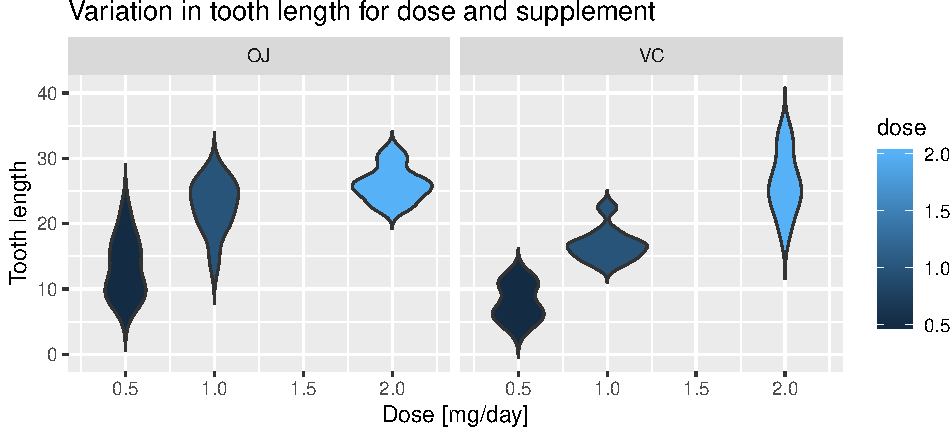
\includegraphics{Basic_Inferential_Data_Analysis_-_Tooth_Growth_files/figure-latex/unnamed-chunk-4-1.pdf}
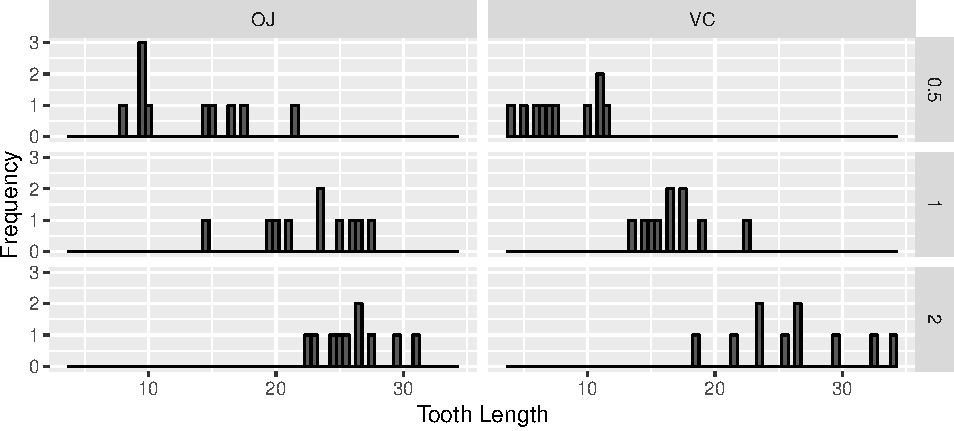
\includegraphics{Basic_Inferential_Data_Analysis_-_Tooth_Growth_files/figure-latex/unnamed-chunk-4-2.pdf}

The violin and histogram figure may indicate that the tooth growth is
higher for larger doses and for the supplement type orange juice (OJ).
This cannot be concluded with any confidence before we have done any
hypothesis testing.

The plots above show that the variances for the different groups
(defined by supplement type and dosage) are not equal. It is also
evident that it cannot be concluded that the variables are normally
distributed, due to the small sample size.

\subsection{Assumptions}\label{assumptions}

\begin{itemize}
\tightlist
\item
  The group can be treated as independent with unequal variances. It
  should be reasonable to consider the groups different since the study
  involved 60 different guinea pigs.
\item
  A confidence interval can be created by applying the t distribution.

  \begin{itemize}
  \tightlist
  \item
    The t distribution is useful for small sample size comparisons and
    assumes normality (but is robust to this assumption within limits).
  \item
    The t distribution will be applied with unequal variances, as
    implied by the violin graph above.
  \item
    The t distribution will be applied without pairing since the data
    contains result for 60 different guinea pigs.
  \end{itemize}
\item
  When considering the hypothesis that dosage amount affects the tooth
  growth, it is sufficient to compare the largest dose with the lowest
  dose (2 mg/day and 0.5 mg/day).
\item
  When considering the hypothesis that supplement type affects the tooth
  growth, the entire dataset with different dosages can be used - due to
  the same number of observations for each dosage.
\item
  A 95 \% confidence interval will be used in hypothesis test.
\end{itemize}

\subsection{Results}\label{results}

\subsubsection{Effect of Tooth Growth by
Dosage}\label{effect-of-tooth-growth-by-dosage}

Compare tooth growth by dose for each supplement type.

\begin{itemize}
\tightlist
\item
  Supplement type ascorbic acid VC:

  \begin{itemize}
  \tightlist
  \item
    H0: mean for high dose = mean for low dose.
  \item
    H1: mean for high dose != mean for low dose.
  \end{itemize}
\item
  Supplement type orange juice:

  \begin{itemize}
  \tightlist
  \item
    H0: mean for high dose = mean for low dose.
  \item
    H1: mean for high dose != mean for low dose.
  \end{itemize}
\end{itemize}

\begin{verbatim}
## [1] -21.90151 -14.41849
## attr(,"conf.level")
## [1] 0.95
\end{verbatim}

\begin{verbatim}
## [1] -16.335241  -9.324759
## attr(,"conf.level")
## [1] 0.95
\end{verbatim}

The t.test shows that for both supplement types the high dose had a
higher tooth growth than the low dose (at 95\% confidence). This can be
concluded since the interval is entirely below zero (as an example).

\subsubsection{Effect of Tooth Growth by Supplement
Type}\label{effect-of-tooth-growth-by-supplement-type}

Compare tooth growth by supplement type.

\begin{verbatim}
## [1] -0.1710156  7.5710156
## attr(,"conf.level")
## [1] 0.95
\end{verbatim}

The t.test shows that it cannot be concluded with 95\% confidence that
orange juice (OJ) leads to more tooth growth than ascorbic acid (VC).

\pagebreak

\section{Appendix: R code}\label{appendix-r-code}

\subsection{Summary of Data}\label{summary-of-data-1}

\begin{Shaded}
\begin{Highlighting}[]
\CommentTok{# Show the distribution of the variables.}
\KeywordTok{summary}\NormalTok{(ToothGrowth)}
\end{Highlighting}
\end{Shaded}

\begin{Shaded}
\begin{Highlighting}[]
\CommentTok{# Dimensions of data}
\KeywordTok{dim}\NormalTok{(ToothGrowth)}
\end{Highlighting}
\end{Shaded}

\begin{Shaded}
\begin{Highlighting}[]
\NormalTok{## Seperate based on dose and supplement type, show mean and 95 % conf interval.}
\CommentTok{# Create ggplot}
\NormalTok{g <-}\StringTok{ }\KeywordTok{ggplot}\NormalTok{(ToothGrowth, }\KeywordTok{aes}\NormalTok{(}\DataTypeTok{x =}\NormalTok{ dose, }\DataTypeTok{y =}\NormalTok{ len, }\DataTypeTok{group =}\NormalTok{ dose))}
\CommentTok{# Violin plot}
\NormalTok{g <-}\StringTok{ }\NormalTok{g }\OperatorTok{+}\StringTok{ }\KeywordTok{geom_violin}\NormalTok{(}\KeywordTok{aes}\NormalTok{(}\DataTypeTok{fill =}\NormalTok{ dose), }\DataTypeTok{trim =} \OtherTok{FALSE}\NormalTok{)}
\CommentTok{# Grid with supplement type in different window}
\NormalTok{g <-}\StringTok{ }\NormalTok{g }\OperatorTok{+}\StringTok{ }\KeywordTok{facet_grid}\NormalTok{(. }\OperatorTok{~}\StringTok{ }\NormalTok{supp)}
\CommentTok{# Create labels}
\NormalTok{g <-}\StringTok{ }\NormalTok{g }\OperatorTok{+}\StringTok{ }\KeywordTok{labs}\NormalTok{(}
  \DataTypeTok{x =} \StringTok{"Dose [mg/day]"}\NormalTok{, }
  \DataTypeTok{y =} \StringTok{"Tooth length"}\NormalTok{, }
  \DataTypeTok{title =} \StringTok{"Variation in tooth length for dose and supplement"}\NormalTok{)}
\CommentTok{# Show plot}
\NormalTok{g}
\end{Highlighting}
\end{Shaded}

\begin{Shaded}
\begin{Highlighting}[]
\CommentTok{# Seperate based on dose and supplement type, show mean and 95 % conf interval.}
\NormalTok{plot <-}\StringTok{ }\KeywordTok{ggplot}\NormalTok{(ToothGrowth, }\KeywordTok{aes}\NormalTok{(len))}
\CommentTok{# Histogram}
\NormalTok{plot <-}\StringTok{ }\NormalTok{plot }\OperatorTok{+}\StringTok{ }\KeywordTok{geom_histogram}\NormalTok{(}\DataTypeTok{color =} \StringTok{"black"}\NormalTok{, }\DataTypeTok{binwidth =} \FloatTok{0.5}\NormalTok{)}
\CommentTok{# Grid wich seperates based on dosage and supplement type}
\NormalTok{plot <-}\StringTok{ }\NormalTok{plot }\OperatorTok{+}\StringTok{ }\KeywordTok{facet_grid}\NormalTok{(dose }\OperatorTok{~}\StringTok{ }\NormalTok{supp)}
\CommentTok{# Create labels}
\NormalTok{plot <-}\StringTok{ }\NormalTok{plot }\OperatorTok{+}\StringTok{ }\KeywordTok{labs}\NormalTok{(}
  \DataTypeTok{x =} \StringTok{"Tooth Length"}\NormalTok{, }
  \DataTypeTok{y =} \StringTok{"Frequency"}\NormalTok{) }
\CommentTok{# Show plot}
\NormalTok{plot}
\end{Highlighting}
\end{Shaded}

\subsection{Assumptions}\label{assumptions-1}

\subsection{Results}\label{results-1}

\subsubsection{Effect of Tooth Growth by
Dosage}\label{effect-of-tooth-growth-by-dosage-1}

\begin{Shaded}
\begin{Highlighting}[]
\NormalTok{## Calculate t.test to see if the hypothesis that }
\NormalTok{## the mean for high and low dose is the same.}
\CommentTok{# Create a subset of dataset without the dosage 1 mg/day.}

\CommentTok{# First, subset with only VC and dosages 0.5 and 2 mg/day.}
\NormalTok{ToothGrowthSuppVC <-}\StringTok{ }\NormalTok{ToothGrowth }\OperatorTok\StringTok{ }
\StringTok{  }\KeywordTok{filter}\NormalTok{(supp }\OperatorTok\StringTok{ "VC"}\NormalTok{) }\OperatorTok\StringTok{ }
\StringTok{  }\KeywordTok{filter}\NormalTok{(dose }\OperatorTok\StringTok{ }\KeywordTok{c}\NormalTok{(}\FloatTok{0.5}\NormalTok{, }\DecValTok{2}\NormalTok{))}

\CommentTok{# Second, subset with only OJ and dosages 0.5 and 2 mg/day.}
\NormalTok{ToothGrowthSuppOJ <-}\StringTok{ }\NormalTok{ToothGrowth }\OperatorTok\StringTok{ }
\StringTok{  }\KeywordTok{filter}\NormalTok{(supp }\OperatorTok\StringTok{ "OJ"}\NormalTok{) }\OperatorTok\StringTok{ }
\StringTok{  }\KeywordTok{filter}\NormalTok{(dose }\OperatorTok\StringTok{ }\KeywordTok{c}\NormalTok{(}\FloatTok{0.5}\NormalTok{, }\DecValTok{2}\NormalTok{))}

\CommentTok{# Perform t.test without paring and assuming unequal variance.}
\KeywordTok{t.test}\NormalTok{(len }\OperatorTok{~}\StringTok{ }\NormalTok{dose, }\DataTypeTok{paired =} \OtherTok{FALSE}\NormalTok{, }\DataTypeTok{var.equal =} \OtherTok{FALSE}\NormalTok{, }\DataTypeTok{data =}\NormalTok{ ToothGrowthSuppVC)}
\KeywordTok{t.test}\NormalTok{(len }\OperatorTok{~}\StringTok{ }\NormalTok{dose, }\DataTypeTok{paired =} \OtherTok{FALSE}\NormalTok{, }\DataTypeTok{var.equal =} \OtherTok{FALSE}\NormalTok{, }\DataTypeTok{data =}\NormalTok{ ToothGrowthSuppOJ)}
\end{Highlighting}
\end{Shaded}

\subsubsection{Effect of Tooth Growth by Supplement
Type}\label{effect-of-tooth-growth-by-supplement-type-1}

\begin{Shaded}
\begin{Highlighting}[]
\CommentTok{# Calculate t.test to see if the hypothesis that the }
\CommentTok{# mean for supplement types are the same.}
\KeywordTok{t.test}\NormalTok{(len }\OperatorTok{~}\StringTok{ }\NormalTok{supp, }\DataTypeTok{paired =} \OtherTok{FALSE}\NormalTok{, }\DataTypeTok{var.equal =} \OtherTok{FALSE}\NormalTok{, }\DataTypeTok{data =}\NormalTok{ ToothGrowth)}
\end{Highlighting}
\end{Shaded}


\end{document}
